% Custom commands
\DefineBibliographyStrings{english}{%
  bibliography = {References},
}


% Redefine how the chapter and section marks are set
%\renewcommand{\chaptermark}[1]{%
%  \markboth{#1}{} % Set left mark to Chapter Title only
%}

\newcommand{\HRule}{\rule{\linewidth}{0.5mm}} 


\newcommand{\ngsolve}{
  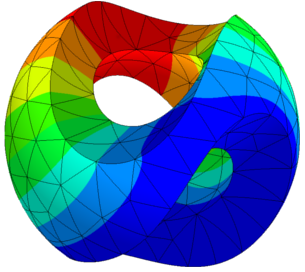
\includegraphics[height=1.25\fontcharht\font`A]{figures/pngs/ngsolvelogo.png}%
  \text{NGSolve }}
 
\newcommand{\extDer}{\boldsymbol{\mathrm{d}}}
\newcommand{\extCoDer}{\boldsymbol{\delta}}
\newcommand{\pref}[1]{(\ref{#1})}

\newcommand{\silnit}{\mathrm{SiN}}
\newcommand{\fatsig}{\boldsymbol{\sigma}}
\newcommand{\fateps}{\boldsymbol{\varepsilon}}
\newcommand{\fateps}{\bm{\epsilon}}
\newcommand{\fatx}{\mathbf{x}}
\newcommand{\fatu}{\mathbf{u}}
\newcommand{\fatv}{\mathbf{v}}
\newcommand{\faty}{\mathbf{y}}
\newcommand{\fatA}{\mathbf{A}}
\newcommand{\fatC}{\mathbf{C}}
\newcommand{\fatM}{\mathbf{M}}
\newcommand{\gold}{\mathrm{Au}}
\newcommand{\chro}{\mathrm{Cr}}
\newcommand{\domainheight}{5.5cm}



% Define Theorem-like Environments
\theoremstyle{plain} % Italicized text
\newtheorem{theorem}{Theorem}[section] % Numbered within sections
\newtheorem{lemma}[theorem]{Lemma} % Shares numbering with Theorem
\newtheorem{corollary}[theorem]{Corollary} % Shares numbering with Theorem

\theoremstyle{definition} % Normal text
\newtheorem{definition}[theorem]{Definition}
\newtheorem{remark}[theorem]{Remark}





